\section{Background}
In this section we will go from Feedforward Neural Networks (FFNs) to the transformer model.


\subsection{Feedforward Neural Networks}
The goal of a Neural Network is to approximate a unknown function $f$ that is
dependent on some variables $\textbf{x}$ and has some output $\textbf{y}$. The 
approximation function $\hat{f}$ is in addition to be dependent on the variables
$\textbf{x}$ also dependent on some parameters $\theta$. Varying these parameters
will change the output of the function $\hat{f}$, and therefor the goal is to find the
parameters that best approximate the function $f$. 


\begin{figure}[h!]
    \centering %Centers the figure
    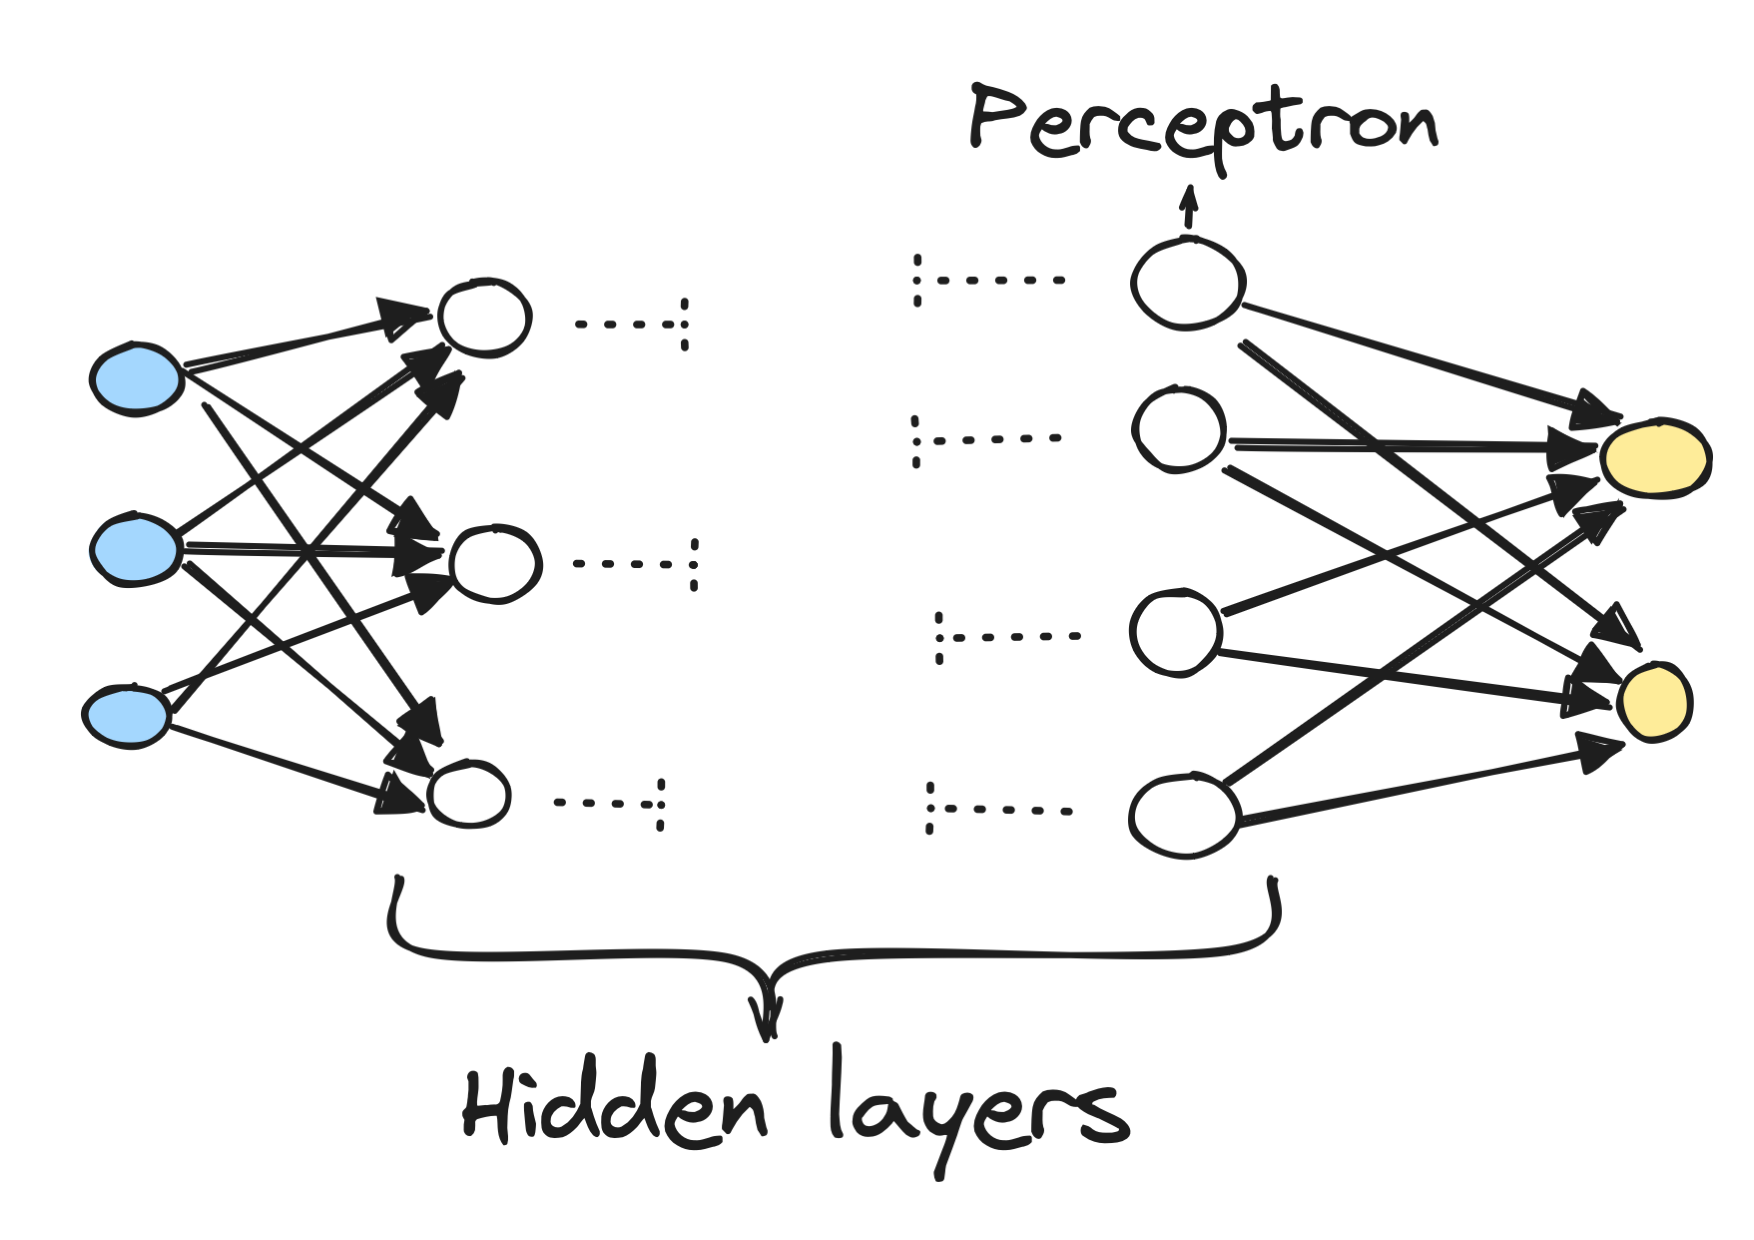
\includegraphics[scale=0.25]{../figs/FNN.pdf} %Imports the figure.
    \caption{Illustration of a fully-connected FNN. The blue dots (on the left) represents the input, where as the yellow 
    (on the right) represents the output. In the middle we find the hidden layers, which can vary both in number, and number of containing perceptrons} %Short explanation of the figure.
    \label{fig:FNN}
\end{figure}


Feedforward Neural Networks can mathematically be seen as a series of 
affine matrix-matrix and matrix-vector multiplications. Another name for FNN is
Multi layer perceptron (MLP). This name gives some insight to the structure of the
network. A perceptron is inspired by the neurons in the human brain. The perceptron
is its own function that takes some inputs, multiplies each input with a weight and
sums the results. This sum together with a bias is then passed through an activation function.
Mathematically this can be written as:
\begin{equation}
    o = a(\sum_{j=1}^{n} w_j i_j + b),
    \label{eq:perceptron}
\end{equation}
where $o$ is the output, $a$ is the activation function, $w_j$ is the weight of input $j$, $i_j$ is the input $j$ and $b$ is the bias.
A neural network is a series of perceptrons, where the output of one layer is the input of the next layer.
Each layer often consist of a number of perceptrons, "stacked" on top of each other.
An illustration of a FNN is presented in Figure \ref{fig:FNN}, where the blue dots represents the input, the yellow the output and the hidden layers in the middle.
Each line between the perceptrons represents a weight, and the bias is not shown in the figure. The white 
circles in the figure represents the activation function of the perceptron, as seen in equation (\ref{eq:perceptron}).

The sum of all the different weights and biases in the network is the parameters of the network, 
referred to as $\theta$. The activation function is what allows the network to learn non-linear functions.
The activation function form can take many forms like the sigmoid function, the tanh function or the ReLU function \cite{Goodfellow-et-al-2016}.

When a FNN/MLP is set up with multiple perceptrons, and the weights are initialized,
the network can given som input values $\textbf{x}$ produce an output $\hat{\textbf{y}}$.
The output is then compared to some "true output" $\textbf{y}$, given by data we have.
With a loss function at hand we can then compute the loss of the network, and use this to update the weights of the network.
The loss function is a measure of how "accurate" the networks prediction of the output is,
and the specific loss function is a choice. The choice of loss function is dependent on the task,
and data at hand. Some common loss functions are the mean squared error and the cross entropy loss \cite{Goodfellow-et-al-2016}.
In the loss function we can also add a regularization term. This can prevent the network from overfitting the data.

Optimization is a crucial step in training neural networks. 
The goal of optimization is to find the set of parameters that minimize a given loss function. 
In the context of neural networks, this typically involves adjusting the weights and biases of the network to minimize the difference between the predicted output and the true output.
There are various optimization algorithms available, such as gradient descent, which iteratively updates the parameters in the direction of steepest descent of the loss function.
Other advanced optimization algorithms, such as Adam and RMSprop, incorporate adaptive learning rates to improve convergence speed. 
Choosing the right optimization algorithm and tuning its hyperparameters can greatly impact the performance of the neural network.

Backpropagation is a key algorithm for training neural networks. 
It is used to compute the gradients of the loss function with respect to the parameters of the network. 
The idea behind backpropagation is to propagate the error from the output layer back to the input layer, updating the weights and biases along the way.
This is done by applying the chain rule of calculus to compute the partial derivatives of the loss function with respect to each parameter.
Backpropagation allows the network to learn from its mistakes and adjust its parameters accordingly.
It is an efficient way to compute the gradients in neural networks with multiple layers and complex architectures. 

The training of a neural network is an iterative process that involves feeding input data through the network,
computing the output, calculating the loss, and updating the parameters using the optimization algorithm 
and backpropagation. This process is repeated for a number of epochs until the network converges to a set of parameters that minimize the loss function.


FNN usecases in NLP is limited by the fact that can not handle sequences of data.
One way to use FNN in NLP is to use a fixed size input, like a bag of words.
This is not ideal, as the order of the words are lost.
We can expand the FNN to handle sequences of data by using Recurrent Neural Networks (RNN).

\subsection{Recurrent Neural Networks}
Recurrent Neural Networks (RNN) are a type of neural network that is designed to handle sequences of data.
This data can be stock prizes over time, audio data or crucially text data.

In opposition to FNN (and also Convolution Neural Networks) where the the outputs only
flow in one direction in, from input towards output. RNNs has connections pointing backwards in the network.
This allows the network to remember information from previous time steps.

The architecture of RRNs can vary heavily. As in the FFNs the number of hidden layers, depth, and 
the number of neurons in each layer, with can be adjusted. In addition to this,
the fact that RRNs can have connections pointing backwards in the network,
additional variations can be made in how these connections are made.

Some design pattern examples from Goodfellow et al. \cite{Goodfellow-et-al-2016} are;
RNNs that have output at every time step and connections between the hidden states.
This means that the hidden state at time step $t$ is connected to the hidden state at time step $t+1$.
Another design could be that the connection only is from the output of the network at time step $t$
is connected to the hidden unit at the next time step $t+1$.
Yet another design mention by Goodfellow et al. is a RRN that takes an entire sequence
as input and produces a single output, where there a connections between the hidden states.

The choice of design is dependent of the task and data at hand. Due to the nature of
the connections in the network it will effect the limitations in prediction and computational demand
in training. For example the first mentioned design, where connections are made between the hidden states,
cannot be trained in parallel, but they exhibit the flexibility that any 
function computable by a Turing machine can be computed a finite size RNN of this design \cite{Goodfellow-et-al-2016}.

Another way of categorizing RNNs, presented in the lectures, is how input and 
output takes form. The four categories are:
\begin{itemize}
    \item One-to-many,
    \item Many-to-one,
    \item Many-to-many (with same length input and output),
    \item Many-to-many (with different length input and output).
\end{itemize}
One-to-many means that the input is a sequence, consisting of only one element,
and the output is a sequence (aka many elements). The rest is self-explanatory. But with a difference in the last two,
some RNNs can have a different length of input and output. As we will see later
RNNs can be used as building blocks, and combined.
\newline

One could think that one is gone, from list of RNNs.
The one-to-one. 
But this one, is one that belong in the list of FNNs. 


\subsubsection{Basic RNNs}

A problem faced when training such RNNs is the vanishing gradient problem.
This problem arises when the gradients of the loss function with respect to the parameters of the network
become very small, making it difficult to update the parameters effectively.
This can occure in FFNs as well, but since
the networks often are limited in depth and with clever choice of activation function an such as the 
ReLU function, it can be avoided. 
RNN's on the other hand are often very deep, they can be made to handle sequences of data of any length,
the vanishing gradient problem is a common issue in training RNNs. In the backpropegation algorithm the gradients are multiplied
due to the chain rule of calculus. If the gradients are small, the product of the gradients will be very small.
This opposite effect, exploding gradients, can happen if the gradients are very large.

Another problem basic RNNs inhabit is the ability to use information from a far away
time step back, to the current time step. 

%%TODO: Mathematically explain the vanishing gradient problem.

\subsubsection{Bidirectional RNNs}

Bidirectional RNNs are a special type of RNNs, categorized by their special connections.
In this networks the output of one time step $t$, depend not only on
the input at time step $t$, like FNNs. Not only on the input at time step $t$ and
previous time steps $t-1, t-2, \dots$, like basic RNNs. But also on the input at time step $t+1, t+2, \dots$.

In bidirectional RNNs, two "sub" RNNs are combined. One that reads the input sequence from left to right,
and one that reads the input sequence from right to left. The networks are
connected such that a output at time step $t$ is dependent on both the
left-to-right sub RNN and the right-to-lef sub RNN.

\subsubsection{Encoder-Decoder Architechture}

The Encoder-Decoder architechture can also be understood by decomposing the network into two parts.
As the name proposes, these parts are called  the encoder and the decoder. Both the 
encoder and the decoder are RNNs.
Given a input sequence $\textbf{X} = (\textbf{x}_1, \textbf{x}_2, \dots ,\textbf{x}_n)$, 
the encoder produces a representation, $C$, of the input sequence. The representation 
could be a single vector, or a sequence. 
Usually a simply function of the last hidden states of the encoder creates $C$ \cite{Goodfellow-et-al-2016}.

Now this representation is passed to the decoder. The decoder 
RNN is trained and architectured to predict a output sequence,
given the representation $C$ of the input sequence.  The great flexibility with the Encoder-Decoder architechture is that
the sequence input and the output sequence can have different lengths,
and they can vary in length as well. 

\subsubsection{Problems with RNNs}

Although RRNs provide much more flexibility and power then FNNs, especially
when working with sequences of data, they still have limitations.

One of them is capturing long-term dependencies. This arises from the 
vanishing gradient problem \cite{MHJ_lecture_notes_W1}. 
The exist architechtures that try to solve this. 
Gated Recurrent Units (GRUs) and Long Short-Term Memory (LSTM) are two examples of this \cite{Goodfellow-et-al-2016}.
These are on the other hand far more complex and computationally demanding.

As shown in this section the sequential nature of RNNs also
makes it hard to find parts to parallelism in the training of the network. Yet another 
huge drawback.


\subsection{Transformers}

The transformer architechture was introduced in the paper 
"Attention is all you need" by Vaswani et al. in 2017 \cite{vaswani2023attention}.
The transformer model is a type of neural network that is based on the self-attention mechanism.
It is structured in a encoder and decoder, the idea being somewhat similar to the Encoder-Decoder architechture of RNNs discussed earlier.
The encoder is responsible for processing the input sequence, turning it into a sequence of hidden states.
It takes a sequence $\textbf{x}$ of length $n$, $\textbf{x} = (x_1, x_2, \dots, x_n)$,
and produces a sequence with equal length $n$ of hidden states $\textbf{h}$, $\textbf{h} = (h_1, h_2, \dots, h_n)$.

In the decoder, the hidden states produced by the Encoder
are connected at a specific point in the decoder (as input).
Then the decoder produces one output at a time, and the output is used as input in the next time step.
The architechture is illustrated in Figure \ref{fig:attention}. We will not explain in detail 
all parts of the model, but we will highlight some key features.

\begin{figure}[h!]
    \centering %Centers the figure
    \includegraphics[scale=0.4]{../figs/attention.pdf} %Imports the figure.
    \caption{The architechture of the Transformer model. Presented in- and obtained from the original paper \cite{vaswani2023attention}.} %Short explanation of the figure.
    \label{fig:attention}
\end{figure}

Part of the innovation that Vaswani et al. introduced was the scaled dot-product attention mechanism.
This mechanism works by having three matrices named 
Query, Value and Key. These are weights of the model,
and are tuned during training as regular weights.
The scaled dot-product attention mechanism can be written as:

\begin{equation}
    \label{scaled_attention}
    \text{Attention}(Q, K, V) = \text{softmax}(\frac{QK^T}{\sqrt{d_k}})V.
\end{equation}

$Q$ is the Query matrix, $K$ is the Key matrix, $V$ is the Value matrix and $d_k$ is the dimension of the Key matrix.
The reason for the named \textit{scaled} dot-product con be seen in equation \ref{scaled_attention},
where the expression $QK^T$ is divided by $\sqrt{d_k}$  before the softmax function is applied.
The benefits from this can be read in the paper \cite{vaswani2023attention}.

Another key feature is the multi-head attention mechanism. This mechanism is a way to allow the model to focus on different parts of the input sequence.
The way this is performed is by linearly project the Query, Key and Value matrices $h$ times, where $h$ is the number of heads.
The projection is learned during trining, and the scaled dot-product attention mechanism is applied to each of the projected matrices.
After each head has produced a output, the outputs are concatenated and linearly projected to produce the final output.
The addition of multi-head attention allows the model to learn different features of the input sequence in parallel \cite{vaswani2023attention}.
It also adds new weights to the model, to perform the linear reduction and , which are tuned during training.

The computation of the Scaled Dot-Product Attention and the Multi-Head Attention is illustrated in Figure \ref{fig:scaleddotproduct_and_multihead}.


\begin{figure}[h!]
    \centering %Centers the figure
    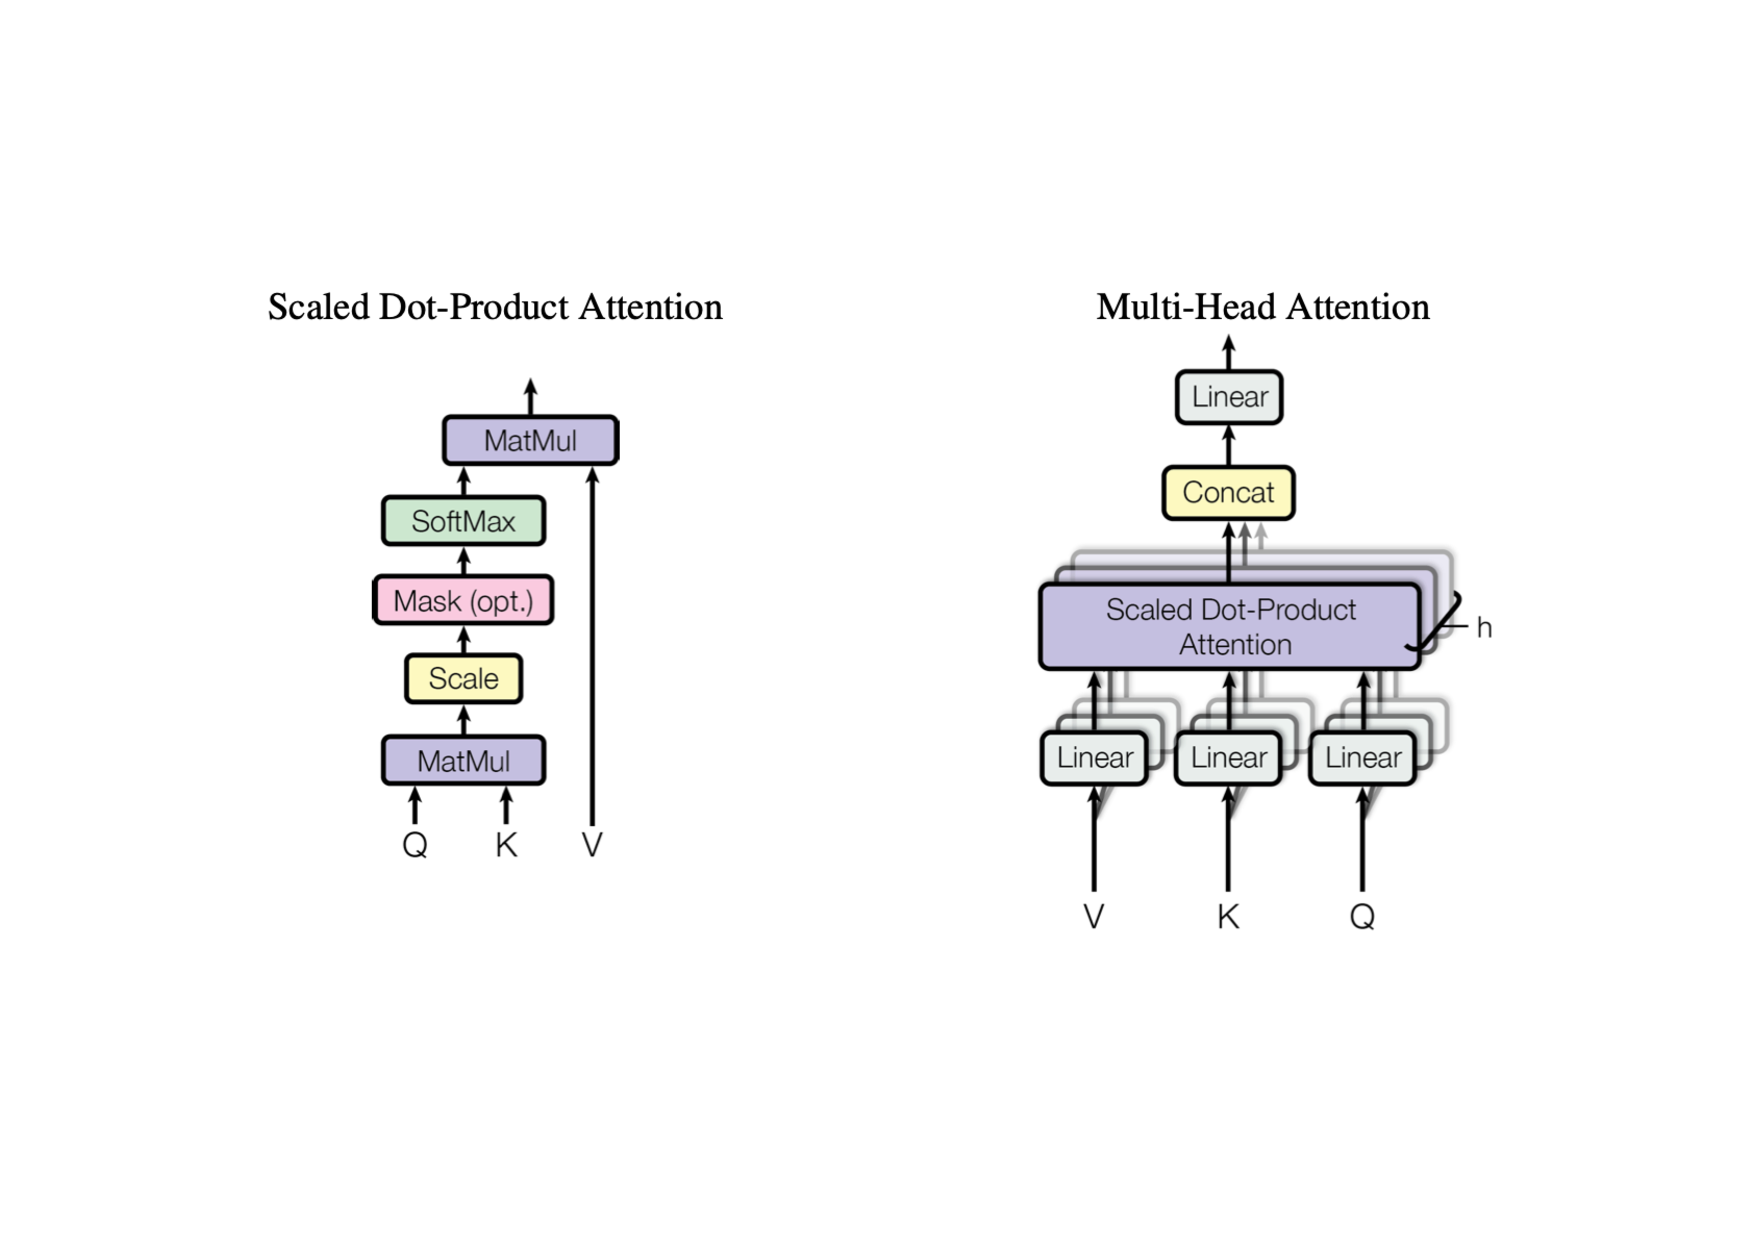
\includegraphics[scale=0.3]{../figs/Scaled_mulit_head.pdf} %Imports the figure.
    \caption{Schematics of the computation of the Scaled Dot-Product Attention as well as how they combine into the Mulit-Head Attention. Also presented in- and obtained from the original paper \cite{vaswani2023attention}.} %Short explanation of the figure.
    \label{fig:scaleddotproduct_and_multihead}
\end{figure}

In addition the model consist of feedforward neural networks, like described previously. It also has layer normalization,
which include taking the mean and variance of the input and normalize it.

This section has highlighted some key features of the transformer model, and how it differs from traditional RNNs.
There is much more to be said, but we will end it here. For more detail please refer to the original paper \cite{vaswani2023attention}.

\subsubsection{BERT}

BERT, which stands for Bidirectional Encoder Representations from Transformers,
represents a significant advancement in the field of NLP. 
Introduced by Devlin et al. in $2019$, BERT is designed to pre-train 
deep bidirectional representations by jointly conditioning on both left and right context
in all layers, which is a departure from previous unidirectional models like GPT.
This bidirectional approach allows BERT to capture more nuanced information from the surrounding context,
resulting in improved performance across a variety of NLP tasks without requiring substantial
task-specific architecture modifications \cite{devlin2019bert}.

The core innovation of BERT lies in its use of the masked language model (MLM)
and next sentence prediction (NSP) pre-training objectives.
The MLM involves randomly masking some of the tokens in the input sequence 
and training the model to predict these masked tokens based on their context. 
Specifically, $15\%$ of the tokens in each sequence are chosen at random to be masked. 
For the chosen tokens, $80\%$ of the time they are replaced with a special [MASK] token, 
$10\%$ of the time they are replaced with a random token, and $10\%$ of the time they remain unchanged. 
This strategy helps the model learn to predict the masked words by using the bidirectional context, 
allowing it to understand the entire context around a word. The MLM objective can be mathematically expressed as:

\begin{equation}
    \label{eq:mlm}
    L_{\text{MLM}} = - \sum_{i \in M} \log P(x_i | x_{\backslash M}),
\end{equation}

where $M$ is the set of masked positions, $x_i$ is the original token at position $i$, and $x_{\backslash M}$ represents the input sequence with the masked tokens.


The NSP task involves predicting whether a given pair of sentences is sequentially coherent,
which helps the model understand the relationship between sentence pairs.
During pre-training, $50\%$ of the time, the second sentence in the pair is the actual next sentence, 
and $50\%$ of the time, it is a random sentence from the corpus.
This task is crucial for improving the model's performance on tasks that require an understanding of the relationship between sentences, 
such as question answering and natural language inference \cite{devlin2019bert}.

BERT's architecture is based on the Transformer model, specifically utilizing the encoder part of the transformer. 
It comes in two primary versions: BERTBASE and BERTLARGE, differing in the number of layers, hidden units, and attention heads. 
BERTBASE consists of $12$ layers, $768$ hidden units, and $12$ attention heads, while BERTLARGE has $24$ layers, $1024$ hidden units, and $16$ attention heads.
This structure allows BERT to handle complex language tasks by providing a deep, 
richly contextualized representation of words and sentences, which can then be fine-tuned on specific tasks such as question answering, sentiment analysis, and named entity recognition \cite{devlin2019bert}.

One of the key advantages of BERT is its ability to be fine-tuned for a variety of downstream tasks with minimal architectural changes. 
During fine-tuning, the pre-trained BERT model is simply extended with an additional output layer appropriate for the task at hand, and the entire model is trained end-to-end. 
This approach significantly reduces the need for task-specific model engineering 
and allows BERT to achieve state-of-the-art performance on a wide range of NLP 
benchmarks, 
such as the General Language Understanding Evaluation (GLUE) benchmark, 
the Stanford Question Answering Dataset (SQuAD), and more \cite{devlin2019bert}.

The impact of BERT on the field of NLP has been profound. 
By providing a robust, pre-trained model that can be easily adapted to various tasks,
BERT has democratized access to powerful NLP capabilities. 
Researchers and practitioners can leverage BERT to improve the accuracy and 
efficiency of their models without needing extensive computational resources or 
specialized knowledge. This has led to a surge in the development and deployment of NLP applications across industries, 
further advancing the capabilities and accessibility of AI-driven language understanding \cite{devlin2019bert}.